\documentclass[xcolor=dvipsnames,table]{beamer}

\usepackage{latexsym}
\usepackage[utf8]{inputenc}
\usepackage[brazil]{babel}
\usepackage{amssymb}
\usepackage{amsmath}
\usepackage{stmaryrd}
\usepackage{fancybox}
\usepackage{datetime}
\usepackage[T1]{fontenc}
\usepackage{graphicx}
\usepackage{graphics}
\usepackage{url}
\usepackage{algorithmic}
\usepackage{algorithm}
\usepackage{acronym}
\usepackage{array}

\usepackage{listings}
\usepackage{color}

\definecolor{mygreen}{rgb}{0,0.6,0}
\definecolor{mygray}{rgb}{0.5,0.5,0.5}
\definecolor{mymauve}{rgb}{0.58,0,0.82}

\lstdefinelanguage{JavaScript}{
  keywords={typeof, new, true, false, catch, function, return, null, catch, switch, var, if, in, while, do, else, case, break},
  keywordstyle=\color{blue}\bfseries,
  ndkeywords={class, export, boolean, throw, implements, import, this},
  ndkeywordstyle=\color{darkgray}\bfseries,
  identifierstyle=\color{black},
  sensitive=false,
  comment=[l]{//},
  morecomment=[s]{/*}{*/},
  commentstyle=\color{purple}\ttfamily,
  stringstyle=\color{red}\ttfamily,
  morestring=[b]',
  morestring=[b]",
}

\lstset{ %
  backgroundcolor=\color{white},   % choose the background color; you must add \usepackage{color} or \usepackage{xcolor}
  basicstyle=\small,        % the size of the fonts that are used for the code
  breakatwhitespace=false,         % sets if automatic breaks should only happen at whitespace
  breaklines=true,                 % sets automatic line breaking
  captionpos=b,                    % sets the caption-position to bottom
  commentstyle=\color{mygreen},    % comment style
  deletekeywords={...},            % if you want to delete keywords from the given language
  escapeinside={\%*}{*)},          % if you want to add LaTeX within your code
  extendedchars=true,              % lets you use non-ASCII characters; for 8-bits encodings only, does not work with UTF-8
  frame=single,	                   % adds a frame around the code
  keepspaces=true,                 % keeps spaces in text, useful for keeping indentation of code (possibly needs columns=flexible)
  keywordstyle=\color{blue},       % keyword style
  language=HTML,                 % the language of the code
  otherkeywords={*,...},           % if you want to add more keywords to the set
  numbers=left,                    % where to put the line-numbers; possible values are (none, left, right)
  numbersep=5pt,                   % how far the line-numbers are from the code
  numberstyle=\tiny\color{mygray}, % the style that is used for the line-numbers
  rulecolor=\color{black},         % if not set, the frame-color may be changed on line-breaks within not-black text (e.g. comments (green here))
  showspaces=false,                % show spaces everywhere adding particular underscores; it overrides 'showstringspaces'
  showstringspaces=false,          % underline spaces within strings only
  showtabs=false,                  % show tabs within strings adding particular underscores
  stepnumber=1,                    % the step between two line-numbers. If it's 1, each line will be numbered
  stringstyle=\color{mymauve},     % string literal style
  tabsize=2,	                   % sets default tabsize to 2 spaces
  title=\lstname,                   % show the filename of files included with \lstinputlisting; also try caption instead of title
  moredelim=**[is][\color{purple}]{@}{@},
}

\newtheorem{definicao}{Definio}
\newcommand{\tab}{\hspace*{2em}}

\mode<presentation>
{
  \definecolor{colortexto}{RGB}{0,0,0}
 
  \setbeamertemplate{background canvas}[vertical shading][ bottom=white!10,top=white!10]
  \setbeamercolor{normal text}{fg=colortexto} 

  \usetheme{Warsaw}
}

\title{Movimento Retilíneo (Parte 3)} 

\author{
  Esdras Lins Bispo Jr. \\ \url{bispojr@ufg.br}
  } 
 \institute{
  Física para Ciência da Computação \\Bacharelado em Ciência da Computação}
\date{\textbf{24 de janeiro de 2017} }

\logo{
\includegraphics[width=1cm]{images/ufgJataiLogo.png}}

\begin{document}

	\begin{frame}
		\titlepage
	\end{frame}

	\AtBeginSection{
		\begin{frame}{Sumário}%[allowframebreaks]{Sumário}
    		\tableofcontents[currentsection]
    		%\tableofcontents[currentsection, hideothersubsections]
		\end{frame}
	}

	\begin{frame}{Plano de Aula}
		\tableofcontents
		%\tableofcontents[hideallsubsections]
	\end{frame}

%------------------------------------------
\section{Pensamento}
	\begin{frame}{Pensamento}
  		\begin{center}
    		
\includegraphics[width=7cm]{images/pensamento.png}
  		\end{center}
	\end{frame}
	
	\begin{frame}{Pensamento}
		\begin{columns}
			\column{.4\textwidth}  		
		  		\begin{center}
		    		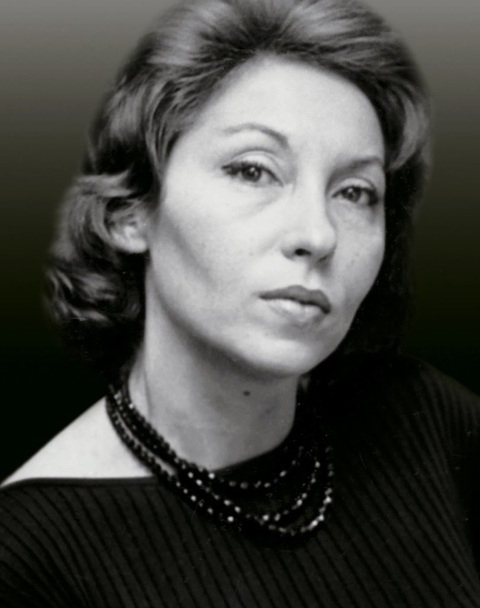
\includegraphics[height=.55\textheight]{images/clarice}
		  		\end{center}
			\column{.6\textwidth}  		
				\begin{block}{Frase}
					\begin{center}
						{\large Mude, mas comece devagar, \\porque a direção é mais importante \\que a velocidade.}
					\end{center}
				\end{block}		  		
		  		\begin{block}{Quem?}
		  			\begin{center}
						{\bf Clarice Lispector (1920-1977)} \\ Escritora ucraniana/brasileira.
					\end{center}
				\end{block}
		\end{columns}
	\end{frame}
	
%------------------------------------------
	\section{Revisão}
	\begin{frame}{Velocidade Instantânea}
		\begin{block}{Velocidade Instantânea}
			\begin{center}
				$v = \underset{\Delta t\rightarrow 0}{\lim} \dfrac{\Delta x}{\Delta t} = \dfrac{dx}{dt}$
			\end{center}
			\begin{itemize}
				\item $v$ também é uma grandeza vetorial.
			\end{itemize}
		\end{block} 
		\begin{block}{Velocidade Escalar Instantânea}
			{\bf Velocidade escalar instantânea}, ou, simplesmente, {\bf velocidade escalar}, é o módulo da velocidade, ou seja, a velocidade desprovida de qualquer indicação de direção ou sentido.
		\end{block}
	\end{frame}

	\begin{frame}{Velocidade Instantânea}
		\begin{block}{Exercício}
			As equações a seguir fornecem a posição $x(t)$ de uma partícula em quatro casos (em todas as equações, $x$ está em metros, $t$ em segundos e $t > 0$): 
				\begin{itemize}
					\item[] (a) Em que caso(s) a velocidade $v$ da partícula é constante?
					\item[] (b) Em que caso(s) a velocidade $v$ é no sentido negativo do eixo $x$?
				\end{itemize}
			\begin{enumerate} 
				\item $x = 3t - 2$
				\item $x = -4t^2 - 2$ 
				\item $x = 2/t^2$ 
				\item $x = -2$ 
			\end{enumerate}
		\end{block}
	\end{frame}

	\section{Movimento Retilíneo (Cont.)}
	
	\begin{frame}{Aceleração}
		\begin{block}{Aceleração Média}
			\begin{center}
				a$_{\mbox{méd}} = \dfrac{\Delta v}{\Delta t} = \dfrac{v_2 - v_1}{t_2 - t_1}$
			\end{center} \pause
			\begin{itemize}
				\item a$_{\mbox{méd}}$ também é uma grandeza vetorial.
			\end{itemize}
		\end{block} \pause
		\begin{block}{Aceleração Instantânea}
			\begin{center}
				a $= \dfrac{d v}{d t}$
			\end{center}
		\end{block} \pause
		\begin{block}{Em outras palavras...}
			Aceleração de uma partícula, em um dado instante, é a {\bf taxa de variação} de velocidade nesse instante.
		\end{block}
	\end{frame}

	\begin{frame}{Exemplo: Aceleração nula}
		\begin{center}
			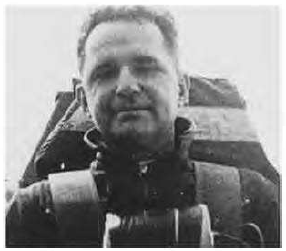
\includegraphics[scale=0.8]{images/fig2-7a}
		\end{center}
	\end{frame}

	\begin{frame}{Exemplo: Aceleração positiva}
		\begin{center}
			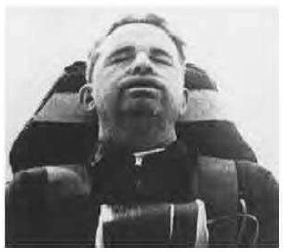
\includegraphics[scale=0.8]{images/fig2-7b}
		\end{center}
	\end{frame}

	\begin{frame}{Exemplo: Aceleração negativa}
		\begin{center}
			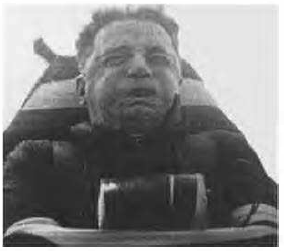
\includegraphics[scale=0.8]{images/fig2-7c}
		\end{center}
	\end{frame}

	\begin{frame}{Aceleração}
		\begin{block}{Logo temos que...}
			\begin{center}
				a $= \dfrac{d v}{d t}$ \pause 
				$ = \dfrac{d}{d t} \left( \dfrac{d x}{d t} \right)$ \pause
				$ = \dfrac{d^2x}{d t^2} $
			\end{center} 
		\end{block} \pause
		\begin{block}{Em palavras...}
			A aceleração de uma partícula em um dado instante é a {\bf derivada segunda} da posição $x(t)$ em relação ao tempo nesse instante.
		\end{block} \pause
		\begin{block}{Unidade no SI}
			$m/s^2$ (metro por segundo ao quadrado)
		\end{block}
	\end{frame}

	\begin{frame}{Elevador: posição $\times$ tempo}
		\begin{center}
			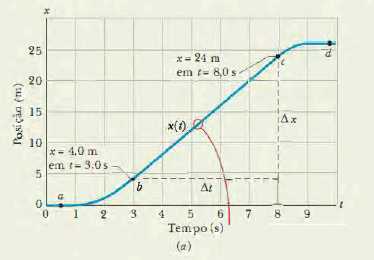
\includegraphics[scale=0.7]{images/fig2-6a}
		\end{center}
	\end{frame}
	
	\begin{frame}{Elevador: velocidade $\times$ tempo}
		\begin{center}
			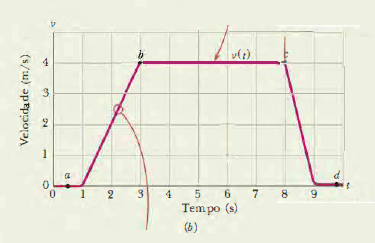
\includegraphics[scale=0.7]{images/fig2-6b}
		\end{center}
	\end{frame}
	
	\begin{frame}{Elevador: $x(t)$ e $v(t)$}
		\begin{center}
			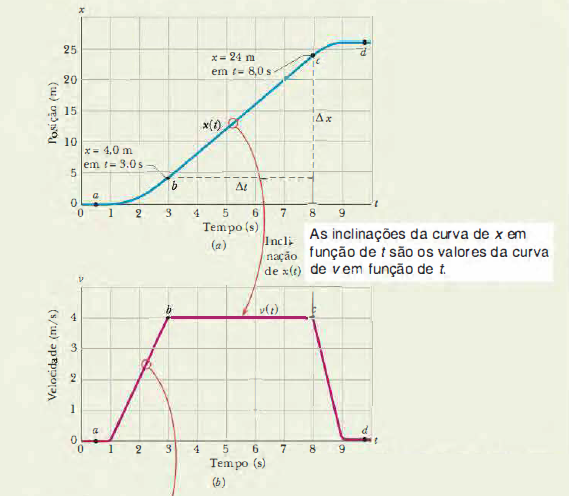
\includegraphics[scale=0.6]{images/fig2-6ab}
		\end{center}
	\end{frame}
	
	\begin{frame}{Elevador: aceleração $\times$ tempo}
		\begin{center}
			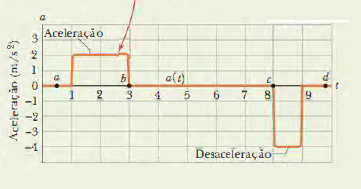
\includegraphics[scale=0.7]{images/fig2-6c}
		\end{center}
	\end{frame}
	
	\begin{frame}{Elevador: $v(t)$ e $a(t)$}
		\begin{center}
			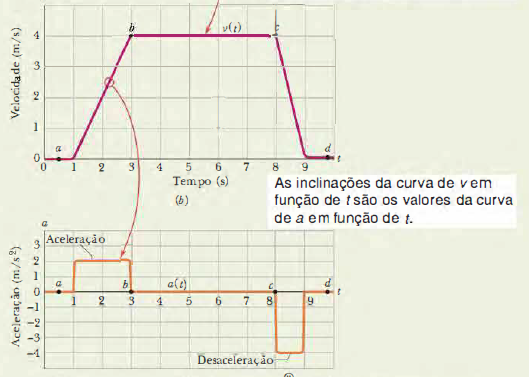
\includegraphics[scale=0.6]{images/fig2-6bc}
		\end{center}
	\end{frame}

	\begin{frame}{Elevador: o que você sentiria?}
		\begin{center}
			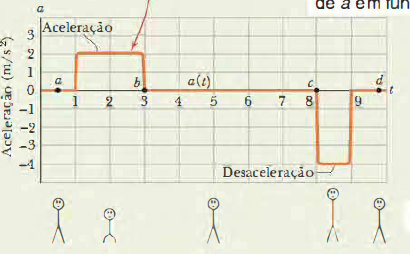
\includegraphics[scale=0.6]{images/fig2-6d}
		\end{center}
	\end{frame}

	\begin{frame}{Aceleração}
		\begin{block}{Normalmente...}
			Grandes acelerações são expressas em unidades $g$:
			\begin{itemize}
				\item $1$ g $= 9,8$ m/s$^2$
			\end{itemize}
		\end{block} \pause
		\begin{block}{Exemplo}
			Montanha russa: $3g$
		\end{block}\pause
		\begin{block}{Aceleração positiva ou negativa?}
			Na disciplina, estes termos referenciarão ao {\bf sentido} e não ao aumento/diminuição de velocidade.
		\end{block}
	\end{frame}

	\begin{frame}{Exemplo}
		\begin{block}{Enunciado}
			Um marsupial se move ao longo do eixo x. Qual é o sinal da aceleração do animal se está se movendo 
			\begin{enumerate}
				\item no sentido positivo com {\bf velocidade escalar} crescente;
				\item no sentido positivo com velocidade escalar decrescente;
				\item no sentido negativo com velocidade escalar
				crescente;
				\item no sentido negativo com velocidade escalar decrescente?
			\end{enumerate}   
		\end{block}
	\end{frame}
	
	\begin{frame}{Velocidade constante}
		\begin{block}{Logo...}
			\begin{center}
				$v_{\mbox{méd}} = v = \dfrac{x - x_0}{t-0}$
			\end{center}
		\end{block} \pause
		\begin{block}{Neste caso...}
			\begin{center}
				$x = x_0 + vt$
			\end{center}
		\end{block}
	\end{frame}
	
	\begin{frame}{Aceleração constante}
		\begin{block}{Logo...}
			\begin{center}
				$a_{\mbox{méd}} = a = \dfrac{v - v_0}{t-0}$
			\end{center} \pause
		Neste caso...
			\begin{center}
				$v = v_0 + at$
			\end{center}
		\end{block} 
	\end{frame}

	\begin{frame}{Aceleração constante}
		\begin{block}{Função x(t)...}
			\begin{center}
				$v_{\mbox{méd}} = \dfrac{x - x_0}{t-0}$
			\end{center}
			Logo...
			\begin{center}
				$x = x_0 + v_{\mbox{méd}}t$
			\end{center}
		\end{block} 
	\end{frame}

		\begin{frame}{Aceleração constante}
		\begin{block}{Entretanto...}
			\begin{center}
				$v_{\mbox{méd}} = \frac{1}{2}(v_0 + v)$
			\end{center}
			Como sabemos que $v = v_0 + at$ temos...
			\begin{center}
				$v_{\mbox{méd}} = \frac{1}{2}(v_0 + v)$ \\
				$v_{\mbox{méd}} = v_0 + \frac{1}{2} at$
			\end{center}
			E temos...
			\begin{center}
				$x - x_0 = v_0t + \frac{1}{2}at^2$
			\end{center}
		\end{block}
	\end{frame}

	


	
	\begin{frame}[shrink]{Bônus (0,5 pt)}
		\begin{block}{Desafio}
			{\bf (Halliday 2.72)} Uma pedra é lançada verticalmente para cima a partir da borda do terraço de um edifício. A pedra atinge a altura máxima 1,60 s após ter sido lançada e, em seguida, caindo paralelamente ao edifício, chega ao solo 6,00 s após ter sido lançada. Em unidades do SI:
			\begin{enumerate}
				\item com que velocidade a pedra foi lançada? 
				\item Qual foi a altura máxima atingida pela pedra em relação ao terraço? 
				\item Qual é a altura do edifício?
			\end{enumerate}
		\end{block}
		\begin{block}{Informações úteis}
			\begin{itemize}
                \item Candidaturas (26 de janeiro, 17h20);
                \item Resposta escrita e apresentação (31 de janeiro, 19h00).
			\end{itemize}
		\end{block} 
	\end{frame}
	
	\begin{frame}
		\titlepage
	\end{frame}
	
\end{document}